%!TEX TS-program = xelatex
\documentclass[]{friggeri-cv}
\usepackage{afterpage}
\usepackage{hyperref}
\usepackage{color}
\usepackage{xcolor}
\hypersetup{
    pdftitle={CV},
    pdfauthor={Afaque},
    pdfsubject={},
    pdfkeywords={},
    colorlinks=false,       % no lik border color
   allbordercolors=white    % white border color for all
}
% \addbibresource{bibliography.bib}
\RequirePackage{xcolor}
\definecolor{pblue}{HTML}{0395DE}

\begin{document}

\header{Afaque}{Hussain}
      {Senior Software Developer}
      
% Fake text to add separator.      
\fcolorbox{white}{gray}{\parbox{\dimexpr\textwidth-2\fboxsep-2\fboxrule}{%
.....
}}

% In the aside, each new line forces a line break.

\begin{aside}
  ~
  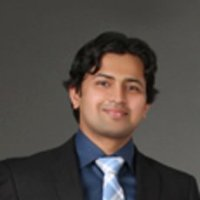
\includegraphics[scale=0.10]{img/me.jpg}
  ~
  \section{Address}
    Espoon Keskus,
    Espoo,
    Finland.
    ~
  \section{Contact}
    +358 46 5374 615
    \href{mailto:Afaque.Hussain@outlook.com}{\textbf{Afaque.Hussain\\@outlook.com}}
    ~
  \section{Web Presence}
    \textbf{Website}
        \href{http://www.afaquehussain.com}{afaquehussain.com}
    ~
    \textbf{GitHub}
        \href{https://github.com/afaquejam}{@afaquejam}
    ~
    \textbf{LinkedIn}
        \href{http://www.linkedin.com/in/afaquejam}{/in/afaquejam}
    ~
  \section{Programming}
    Python, C, C++, Java
    ~
  \section{Familiarity}
    HTML, Javascript,
    PHP, Bash Scripting, ABAP, Assembly
    ~
   \section{Tools/Practices}
     \textbf{Vim, Git, Jenkins, Phabricator, TDD, Agile}
   ~
  \section{OS Preference}
    \textbf{Linux}
\includegraphics[scale=0.40]{img/5stars.png}
    \textbf{Mac OS X}
\includegraphics[scale=0.40]{img/2stars.png}
    \textbf{Windows}
\includegraphics[scale=0.40]{img/1stars.png}
    ~
\end{aside}

\section{Education}
\begin{entrylist}
  \entry
    {2012 - 2015}
    {Master of Science}
    {\Large{University of Helsinki, Finland}}
    {Computer Science, Networking.\\
     {GPA}: \textbf{5/5} \\
     {Master's Thesis}: \emph{WebRTC in presence of NAT, Firewalls and HTTP Proxies.}\\
     {Thesis Supervisor}: \emph{Prof. Jussi Kangasharju.}\\
     \emph{This education is associated with 12 courses, 9 projects and 1 honours and awards.}\\}
  \entry
    {2007 - 2011}
    {Bachelor Of Engineering}
    {\Large{VTU, India}}
    {Computer Science \& Engineering.\\
    \emph{First Class with Distinction in all eight semesters.}\\
    This education is associated with 31 courses, 5 projects, 5 honours and awards.\\}
\end{entrylist}

\section{Experience}
\begin{entrylist}
  \entry
    {06/13 - Now}
    {Software Developer (2 Years)}
    {\Large{Ericsson, Finland}}
    { Working on the Industrial Internet (IoT) cases. Prior to that, worked on addressing the problems of WebRTC in presence of network middle boxes, video transcoding for WebRTC and developement of Ericsson's Social Web of Things. \\
    {\emph{Python, C, GStreamer, Java, Javascript.}\\}}
%   \entry
%     {06/13 - 12/13}
%     {Software Developer Trainee}
%     {Ericsson, Finalnd}
%     {Worked on the development of Ericsson's \href{http://www.youtube.com/watch?v=i5AuzQXBsG4}{Social Web of Things Project}.\\
%     \emph{Java, CoAP, Internet of Things}\\}
  \entry
    {01/13 - 05/13}
    {Software Developer (5 months)}
    {\Large{University of Helsinki}}
    {A collaborative project based software engineering curriculum coordinated by \textbf{Facebook Inc.} and \textbf{Stanford University}. As a part of this project, I was flown to Facebook Headquarters, Menlo Park, California, for a 3 day kick-off Hackathon. Contributed about \textbf{50 patches} to Phabricator, Arcanist and Libphutil open source projects.\\
    \emph{PHP, Phabricator.}\\}
    \entry
    {08/11 - 08/12}
    {Software Engineer (1 Year)}
    {\Large{Philips Electronics}}
    {Worked as a Software Developer in Ultrasound Research \& Development Team, Philips Healthcare. Prior to that, I also worked with Philips IT team creating a Purchase Order Approval System by interfacing Android and SAP systems.\\
    \emph{C++, Java, Android.}\\}
    \entry
    {07/10 - 10/10}
    {Intern  (3 Months)}
    {\Large{Nokia}}
    {Worked on FreOffice (now Calligra Mobile) development, a collaborative effort with KDE developers and Nokia. Developed Optical Character Recognition, Document Translator \& Transliteration support for FreOffice. Researched on developing FreOffice using Qt Creator. The work is published on KDE website: techbase.kde.org/User:Kumarafaque\\
    \emph{C++, Qt, Maemo.}}
\end{entrylist}

% \section{Certifications}
% \begin{entrylist}
%   \entry
%     {02/2013}
%     {Intro to Computer Science}
%     {Udacity. E-learning}
%     {\emph{Building a Python Search Engine}}
% \end{entrylist}

\newpage

\begin{aside}
~
~
~
   \section{Frameworks}
    Qt, GStreamer
~
%   \section{Personal Skills}
%   ~
  \section{Languages}
    \textbf{English}
\includegraphics[scale=0.40]{img/5stars.png}
    \textbf{Hindi}
\includegraphics[scale=0.40]{img/5stars.png}
    \textbf{Finnish}
\includegraphics[scale=0.40]{img/1stars.png}
~
  \section{Hobbies}
    Self Defence, Working-Out,
    Driving, Partying.
~
\section{Legal}
    Age: \textbf{25}
    \textbf{Indian}
    \emph{Work Permit in Finland.}
~
\end{aside}


\section{Other Information}
\begin{itemize}

\item My WebRTC based application \href{http://blog.tadhack.com/2014/06/09/tadhack-winners-madrid-remote3/}{Foosball-CAM} won second prize in TAD HACK hackathon in Madrid, Spain 2014.
\item Gave Tech Talks @ Ericsson on On-line Privacy, TOR Network and WebRTC.
\item Represented Ericsson at the Open Innovation Expo 2013, Moscow, Russia.
\item One of the eight students selected by University of Helsinki for participating in the Facebook Hackathon and Open curriculum course.
\item Identified as Early Career Potential by Philips. One of 22 selected among 13000 applications all over India.
\item Won 1st prize in IEEE Project Competition in Higher End Project Category during undergraduate studies.
\item Won 3rd prize in state level paper presentation during undergraduate studies.
\item Stood 3rd at Regional Levels in TCS Tech Bytes conducted by TCS.
\item Trained 50 students on developing applications using Qt Framework in workshop organized by IEEE held at KLESCET, India.
\item Developer and former Maintainer of an application which is published in Extras-Devel repository of Nokia’s Maemo Operating System. Also, my work has been mentioned in a German Technology Website. Link: http://maemo.soup.io/since/82371119
\item Representative Of Computer Science for IEEE Student Branch during undergraduate studies.
\item ACE(Association of Computer Engineers) Secretary during undergradute studies.
\end{itemize}
~
\section{References}
References will be provided upon request.
~
\section{Projects}
You can visit my \href{http://www.linkedin.com/in/afaquejam}{LinkedIn} and \href{https://github.com/afaquejam}{GitHub} profile to have a look at my projects.
Due to privacy concers, my LinkedIn profile can only be accessed using a LinkedIn account. However, I could make my profile public for a short period time, if you'd like.
\\
\\
\\
\emph{May 25, 2015} \\
\textbf{Afaque Hussain} \\
\\

\includegraphics[scale=0.40]{img/qrcode.png}

\end{document}
